% =========================================================
% CONFIGURACION DEL DOCUMENTO
% =========================================================
\providecommand{\main}{..}
\documentclass[\main/main.tex]{subfiles}

% =========================================================
% CONTENIDO
% =========================================================
\begin{document}
\chapter{Sistema propuesto}
\label{cha:03_sistema_propuesto}
	% ===============================================================
	% ===============================================================
	\section{\textit{Setup} a utilizar}
	\label{sec:03_setup}
		Debido a que este trabajo de memoria corresponde fundamentalmente a una prueba de concepto se decidió junto al profesor guía evitar en lo posible la compra de nuevo equipamiento y por tanto no se entrega particular importancia a cumplir de forma estricta con las características de hardware utilizado en instancias formales de investigación. Con esto en consideración se presenta a continuación una descripción del entorno de hardware y software utilizado:
		\begin{table}[H]\begin{center}\footnotesize{
			\singlespacing{
			\begin{tabular}{| C{0.11\textwidth} | C{0.14\textwidth} | R{0.18\textwidth} L{0.5\textwidth} |} \hline
				\multirow{7}{*}{Hardware} 	& \multirow{4}{*}{PC} 			& Procesador: 		& Intel Core i7-3770 \\
										& 							& Memoria RAM:		& $16.0[GB]$, DDR3, $650[MHz]$ \\
										& 							& Disco duro: 		& Samsung SSD, 840 Series, $120[GB]$ \\
										& 							& Tarjeta gráfica: 	& NVIDIA GeForce GTX 660 Ti, $2[GB]$ \\ \cline{2-4}
										& \multirow{2}{*}{Monitores}& Principal:		& Samsung SyncMaster, $1680\times1050[px]$, $60[Hz]$ \\ 
										& 							& Secundario: 		& Samsung SyncMaster, $1680\times1050[px]$, $60[Hz]$ \\ \cline{2-4}
										& Adquisición 				& \textit{Eye tracker}: 		& EyeTribe \\ \hline
				\multirow{4}{*}{Software} 	& \multirow{2}{*}{Entorno} 		& SO:				& Windows 10 Pro x64 \\ 
										& 							& Base:				& Python 2.7 x86, Anaconda \\ \cline{2-4}
										& \multirow{2}{*}{Módulos}		& Principal: 			& PsychoPy 1.84.2\cite{psychopy} \\
										& 							& Requeridos:			& Ver anexo \ref{cha:a01_instalacion} \\ \hline
			\end{tabular}}
			\caption{Hardware y software utilizado en el desarrollo.}
			\label{tbl:03_hs_selection}
		}\end{center}\end{table}

		\newpage
		La elección de software se encuentra infuenciada fuertemente por los siguientes puntos:
		\begin{enumerate}
			\item El \textit{eye tracker} a utilizar solo tiene disponible sus drivers para Mac y Windows. Debido a la facilidad de encontrar computadoras con Windows se decanta por este \acrshort{so}.

			\item Los desafíos del sistema a implementar requieren del uso de un lenguaje orientado a objetos. A pesar de las bondades de Octave o Matlab en procesamiento y acceso a módulos complementarios estos entornos carecen de buen soporte para este tipo de programación, por este motivo se utiliza Python como lenguaje de desarrollo. 

			\item Dentro de las opciones disponibles PsychoPy resulta sumamente interesante. Cumple con ser open-source, es ampliamente utilizado por investigadores, presenta documentación detallada y clara para todas sus funciones y los foros se encuentran activos. Otro punto interesante es que entrega soporte para varias marcas de \textit{eye tracker}, entre los cuales se encentra el seleccionado.

		\end{enumerate}

	% ===============================================================
	% ===============================================================
	\section{Diseño del sistema}
	\label{sec:03_diseño_sistema}
		El sistema a ser desarrollado en este trabajo de título tiene como función principal facilitar el proceso de configuración y puesta en marcha de experimentos asociados a movimiento ocular. Para esto, se considera oportuno subdividir el desarrollo en tres partes: La primera consiste en determinar la estructura de datos requerida para almacenar tanto las configuraciones del sistema como de las tareas a implementar. La segunda implica la implementación de los métodos de configuración y ejecución del experimento, asegurando su correcto funcionamiento. La tercera etapa corresponde a montar estas funciones en una GUI para facilitar el proceso a personas que no tengan conocimiento del lenguaje. Así, se presenta a continuación el trabajo realizado.

		% ###########################################################
		\subsection{Primera parte: Estructura de datos}
		\label{sub:03_estructura_datos}
			Al diseñar la estructura de datos se debió considerar el problema desde tres aristas. La primera correspondía a la necesidad de almacenar la información del conjunto compuesto por experimento-tareas-cuadros-componentes donde, complementando lo expuesto en el apartado \ref{sub:02_experimentos_de_estimulacion}, las tareas corresponden a las actividades específicas que el sujeto de prueba debe llevar a cabo. Los cuadros corresponden a los elementos que conforman dichas tareas y los componentes serán considerados como las figuras e imágenes contenidas en cada cuadro. La segunda dice relación con la información complementaria que se desea incluir para posterior análisis, tal como comentarios del investigador encargado del experimento para una sesión específica o algunas características de quien realizará el experimento, tales como su edad, sexo, color de ojos o si se utilizan lentes durante la ejecución. Finalmente, la tercera arista implica el conservar las configuraciones del equipo y hardware a utilizar para montar el servicio de ejecución asociado al módulo ioHub, que es el componente de PsychoPy que permite sincronizar todos los dispositivos asociados a la ejecución del experimento: teclado, pantalla, \textit{eye tracker}, etc. y almacenar los datos en un archivo. 
			\begin{figure}[H]
				\centering
				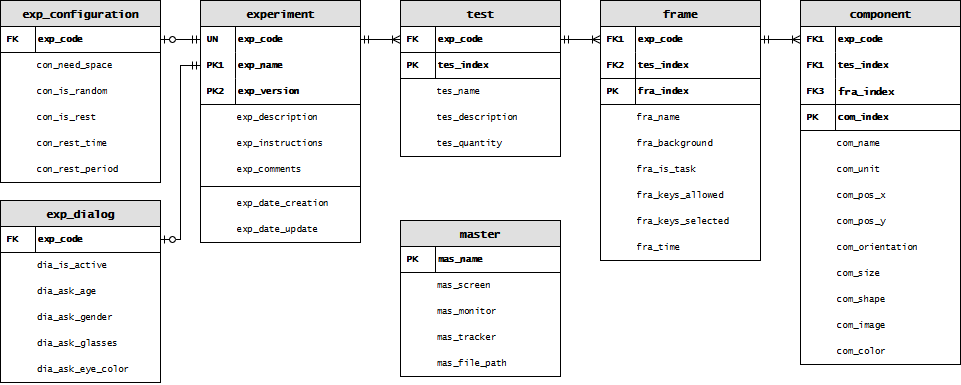
\includegraphics[width=\textwidth]{cap_03_database}
				\caption{Diagrama de base de datos a implementar.}
				\label{fig:03_database}
			\end{figure} 

			En base a lo anterior, se propone como solución el uso de una base de datos local de tipo SQLite con la estructura presentada en la figura \ref{fig:03_database}. A continuación se comenta el contenido de cada tabla y su función:
			\begin{enumerate}
				\item \textbf{master:} Almacena la información asociada a un perfil de configuración del hardware a utilizar. Cada perfil es identificado con un nombre e indica qué pantalla será utilizada (screen), cuál es la configuración de dicha pantalla (monitor, se define en un aplicativo de PsychoPy), qué \textit{eye tracker} se utilizará (tracker) y en qué directorio se almacenará el archivo resultante.

				\item \textbf{experiment:} Almacena la información de identificación de un experimento. Cada experimento se identifica por un código único (code) y un par nombre/versión (name/version), que tiene como objetivo identificar a una aplicación específica de una familia del mismo tipo, por ejemplo: ''antisaccade''/''v1.0\_gap''. Además, se incluye un campo para la descripción, instrucciones para el usuario (instructions) y comentarios para quien tome el experimento (comments). Se incluyen la fecha de creación y la última modificación para dejar de forma explícita una señal de cuidado: Las condiciones del experimento pueden no ser las mismas de la última ejecución.
				
				\item \textbf{exp\_configuration:} Esta tabla es complementaria al experimento y almacena la configuración general de ejecución. \textquestiondown Es necesario que el paciente presione la tecla espacio antes de cada tarea? (need\_space), \textquestiondown El orden de las tareas es aleatorio o secuencial? (is\_random), \textquestiondown Se incluyen en el experimento tiempos de descanso? (is\_rest), \textquestiondown Cada cuántas tareas? (rest\_period), \textquestiondown Con qué duración? (rest\_time).

				\item \textbf{exp\_dialog:} Esta tabla es complementaria al experimento y almacena la configuración del diálogo inicial, que permite obtener información adicional sobre el paciente. \textquestiondown Se incluirá información complementaria? (is\_active), \textquestiondown Qué edad tiene el paciente? (ask\_age), \textquestiondown Cuál es su sexo? (ask\_gender), \textquestiondown Utiliza gafas o lentes de contacto? (ask\_glasses), \textquestiondown Cuál es su color de ojos? (ask\_eye\_color).

				\item \textbf{test:} Esta tabla contiene, para cada experimento, la identificación de las tareas a utilizar. Cada tarea se identifica por su nombre (name) y debe especificar el número de repeticiones a ser ejecutadas (quantity). Incluye un campo para añadir una descripción de la tarea (description).

				\item \textbf{frame:} Esta tabla contiene, para cada tarea, el conjunto de cuadros que la conforman. Cada cuadro se identifica por un nombre (name) y permite la configuración de su comportamiento y características de forma general: color de fondo (color), si el cuadro corresponde a una tarea que requiere respuesta de teclado o es temporizada (is\_task), las teclas habilitadas (keys\_allowed), las teclas que se espera sean presionadas (keys\_selected) y el tiempo por el cual debe ser presentada (time).

				\item \textbf{component:} Esta tabla contiene, para cada cuadro, el conjunto de componentes o elementos que la conforman. Cada componente se identifica por un nombre (name) y las configuraciones asociadas a las unidades de medida consideradas (units), su posición en la pantalla (pos\_x, pos\_y), su tamaño (size), si se encuentra rotada o no (orientation), si es una figura, su forma (shape) y color (color) o si es una imagen el binario correspondiente (image). 
			\end{enumerate}

			Este modelo se considera apropiado por los siguientes motivos:
			\begin{enumerate}
				\item Aísla un experimento de otro al tener tareas y configuraciones completamente independientes. Esta configuración permite evitar que cambios en alguna tarea para ajustarse a necesidades específicas de un experimento afecte el funcionamiento del resto.

				\item No puede existir una tarea que no se encuentre asociada a algún experimento, esto aplica también a cuadros y componentes. 

				\item Tener toda la información y configuraciones contenidas en un archivo facilita la portabilidad y migración desde un equipo a otro. Además, dado que es tratable como una base de datos convencional facilita el proceso de revisión de los datos sin necesidad del programa principal.
			\end{enumerate}

			Cabe destacar que, para asegurar la limpieza de la base de datos se tomo la decisión de generar tanto updates como deletes en cascada a todas las tablas asociadas a un experimento, de esta forma, al eliminar un experimento particular se eliminan también todas sus tareas y configuraciones, evitando data residual. Esto se repite en niveles más bajos también: eliminar una tarea elimina todos sus cuadros, eliminar un cuadro elimina también todos sus componentes.  

		% ###########################################################
		\subsection{Segunda parte: Implementación de las funciones principales}
		\label{sub:03_implementacion_backtend}
			Para lograr sincronizar la ejecución del experimento con el uso de dispositivos tales como el monitor, el teclado y el \textit{eye tracker} se hará uso de ioHub \cite{website:iohub}. IoHub es un módulo que forma actualmente parte de PsychoPy y que fue desarrollado originalmente por Sol Simpson. Su funcionalidad principal consiste en montar un servicio por el cual se hace una revisión constante de los dispositivos de entrada/salida seleccionados, almacenando la información recopilada de forma ordenada en un archivo con formato hdf5, que corresponde a un tipo de diccionario donde se ordenan los datos. Para construir la aplicación en base a esta utilidad se debe generar un conjunto de métodos que permita lograr las funcionalidades presentadas en la figura \ref{fig:03_application_concept}. 
			\begin{figure}[H]
				\centering
				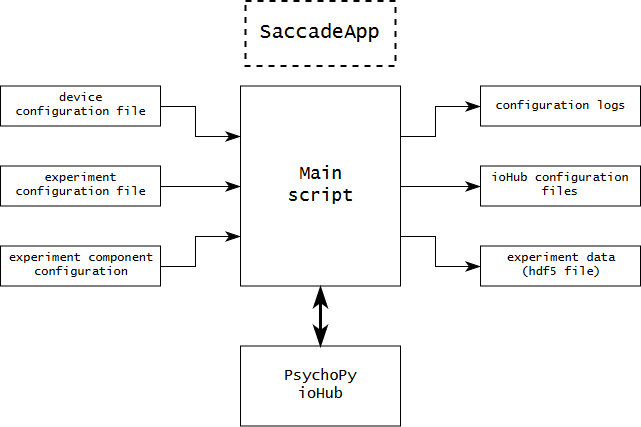
\includegraphics[width=0.7\textwidth]{cap_03_application_concept}
				\caption{Diagrama de funcionamiento general.}
				\label{fig:03_application_concept}
			\end{figure} 

			Para esto, es necesario entregar tres insumos: la configuración de los dispositivos que serán monitorizados por ioHub, la configuración general del experimento (identificadores, descripción y los elementos que conforman las ventanas de diálogo) y la configuración de los elementos asociados a la presentación de estímulo (que se conforman por otras rutinas de PsychoPy).

			En la figura \ref{fig:03_base_class_tree} se presenta la estructura de clases implementada en este trabajo de título. Las clases Master, Experiment, Test, Frame y Component representan el conjunto de funciones que permiten manejar la configuración almacenada en las respectivas tablas de la base de datos además de otorgar otras funcionalidades que se enfocan en la ejecución del experimento propiamente tal. Debido a que Experiment, Test y Frame implican el manejo de una lista de componentes, estas son creadas como clases que heredan las funcionalidades básicas para el manejo de listas como el agregar, copiar o eliminar elementos, cambiar su posición en la lista, etc. La clase utils implementa métodos de formateo de datos, tales como la conversión de strings a formato unicode o el formateo de fechas. SaccadeDB otorga funcionalidades que permiten comunicarse con el archivo de base de datos. Finalmente, la clase ExperimentHandler es la encargada de generar crear las carpetas de almacenamiento, los archivos de respaldo, los logs de configuración y la inicialización de la ejecución del experimento, que es implementado en la clase ExperimentRuntime (que hereda de ioHub e inicia el servicio asociado). La clase Switch implementa una estructura similar a un switch-case con el fin de utilizar una máquina de estados que regule la carga de frames durante la ejecución.  
			\begin{figure}[H]
				\centering
				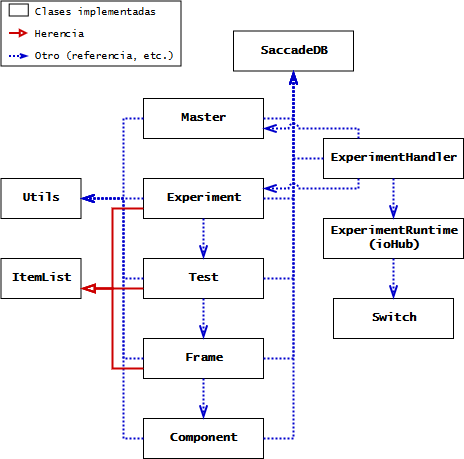
\includegraphics[width=0.6\textwidth]{cap_03_base_class_tree}
				\caption{Diagrama de clases del sistema (no considera GUI).}
				\label{fig:03_base_class_tree}
			\end{figure} 

			\newpage
			A continuación se describe con un mayor grado de detalle cada clase. Por simplicidad se obvian las funciones asociadas al get-set de los atributos (que corresponden a los datos almacenados en la base de datos):
			\begin{enumerate}
				\item \textbf{Utils:} Clase utilizada para implementar funcionalidades de formateo de datos.
				
				\vspace{-8mm}			
				\begin{center}\footnotesize{\singlespacing{
					\begin{longtable}[H]{| C{0.15\textwidth} | R{0.13\textwidth} L{0.6\textwidth} |} \hline
						% ===============================================
						\multicolumn{3}{|c|}{\multirow{2}{*}{\textbf{format\_text}}}\\\multicolumn{3}{|c|}{}\\\hline
						Descripción & \multicolumn{2}{L{0.75\textwidth}|}{
						Método estático. Convierte un string o similar a formato unicode. Si el dato ingresado no cumple con las condiciones de formato se devuelve un elemento vacío.
						}\\\hline
						\multirow{3}{*}{Inputs} & word: 	& String o dato a ser formateado. \\
						 						& lmin: 	& Largo mínimo de la palabra. \\
						 						& lmax: 	& Largo máximo de la palabra. 
						\\\hline
						Return 					& unicode. 	& 
						\\\hline 
						% ===============================================
						\multicolumn{3}{|c|}{\multirow{2}{*}{\textbf{format\_int}}}\\\multicolumn{3}{|c|}{}\\\hline
						Descripción & \multicolumn{2}{L{0.75\textwidth}|}{
						Método estático. Convierte un valor en entero. Si el valor no cumple con las condiciones dadas se devuelve un valor por defecto, especificado por el usuario.
						} \\ \hline
						\multirow{3}{*}{Inputs} & value: 	& Valor a ser formateado. \\
						 						& vmin: 	& Valor mínimo permitido. \\
						 						& default: 	& Valor por defecto. 
						\\\hline
						Return 					& int. 	& 
						\\\hline
						% ===============================================
						\multicolumn{3}{|c|}{\multirow{2}{*}{\textbf{format\_float}}}\\\multicolumn{3}{|c|}{}\\\hline
						Descripción & \multicolumn{2}{L{0.75\textwidth}|}{
						Método estático. Convierte un valor en flotante. Si el valor no cumple con las condiciones dadas se devuelve un valor por defecto, especificado por el usuario.
						}\\\hline
						\multirow{3}{*}{Inputs} & value: 	& Valor a ser formateado. \\
						 						& vmin: 	& Valor mínimo permitido. \\
						 						& default: 	& Valor por defecto. 
						\\\hline
						Return 					& float. 	& 
						\\\hline
						% ===============================================
						\multicolumn{3}{|c|}{\multirow{2}{*}{\textbf{format\_bool}}}\\\multicolumn{3}{|c|}{}\\\hline
						Descripción & \multicolumn{2}{L{0.75\textwidth}|}{
						Método estático. Convierte el valor entregado en un booleano. Si el valor no puede ser convertido se devuelve algún valor por defecto especificado por el usuario.
						}\\\hline
						\multirow{2}{*}{Inputs} & state: 	& Estado a ser formateado. \\
						 						& default: 	& Valor por defecto. 
						\\\hline
						Return 					& bool. 	& 
						\\ \hline
						% ===============================================
						\multicolumn{3}{|c|}{\multirow{2}{*}{\textbf{format\_path}}}\\\multicolumn{3}{|c|}{}\\\hline
						Descripción & \multicolumn{2}{L{0.75\textwidth}|}{
						Método estático. Formatea la dirección entregada dependiendo del sistema operativo.
						}\\\hline
						Inputs 					& path: 	& Dirección a ser formateada. 
						\\\hline
						Return 					& unicode. 	& 
						\\\hline \newpage
						% ===============================================
						\multicolumn{3}{|c|}{\multirow{2}{*}{\textbf{get\_time}}}\\\multicolumn{3}{|c|}{}\\\hline
						Descripción & \multicolumn{2}{L{0.75\textwidth}|}{
						Método estático. Permite convertir un string asociado a una fecha desde el formato de tiempo GTM a el horario de Chile continental. Esta función se agrega debido a la configuración horaria de la base de datos.
						}\\\hline
						Inputs 					& date: 	& String que representa una fecha en formato Y-m-d H:M:S. 
						\\\hline
						Return 					& unicode. 	& 
						\\\hline
					\caption{Métodos implementados en la clase Utils.}
					\label{tbl:03_class_utils}
					\end{longtable}}}
				\end{center}
				
				\vspace{-15mm}
				\item \textbf{SaccadeDB:} Clase utilizada para implementar la conexión con la base de datos SQLite.
				
				\vspace{-8mm}			 
				\begin{center}\footnotesize{\singlespacing{
					\begin{longtable}[H]{| C{0.15\textwidth} | R{0.13\textwidth} L{0.6\textwidth} |} \hline
						% ===============================================
						\multicolumn{3}{|c|}{\multirow{2}{*}{\textbf{SaccadeDB}}}\\\multicolumn{3}{|c|}{}\\\hline
						Descripción & \multicolumn{2}{L{0.75\textwidth}|}{
						Constructor. Inicializa los atributos del objeto.
						}\\\hline
						Inputs 					& filepath: & Ubicación (string o unicode) del archivo de base de datos.
						\\\hline
						Return 					& void. 	& 
						\\\hline 
						% ===============================================
						\multicolumn{3}{|c|}{\multirow{2}{*}{\textbf{connect}}}\\\multicolumn{3}{|c|}{}\\\hline
						Descripción & \multicolumn{2}{L{0.75\textwidth}|}{
						Método que inicia una conexión con el archivo de base de datos. Si el archivo de base de datos epecificado en el constructor no existe, crea uno nuevo utilizando las configuraciones por defecto.
						}\\\hline
						Inputs 					& void. 	&  
						\\\hline
						Return 					& void. 	& 
						\\\hline 
						% ===============================================
						\multicolumn{3}{|c|}{\multirow{2}{*}{\textbf{close}}}\\\multicolumn{3}{|c|}{}\\\hline
						Descripción & \multicolumn{2}{L{0.75\textwidth}|}{
						Método que finaliza, de ser posible, la conexión con la base de datos.
						}\\\hline
						Inputs 					& void. 	&  
						\\\hline
						Return 					& bool. 	& Verdadero si la conexión se cierra apropiadamente, falso en caso contrario.
						\\\hline 
						% ===============================================
						\multicolumn{3}{|c|}{\multirow{2}{*}{\textbf{push\_query}}}\\\multicolumn{3}{|c|}{}\\\hline
						Descripción & \multicolumn{2}{L{0.75\textwidth}|}{
						Método que permite realizar querys que involucran modificar los contenidos de la base de datos (insert, update, delete, etc.).
						}\\\hline
						Inputs 					& query. 	& Instrucción SQL (string o unicode).
						\\\hline
						Return 					& bool. 	& Verdadero si la query se ejecuta correctamente, falso en caso contrario.
						\\\hline 
						% ===============================================
						\multicolumn{3}{|c|}{\multirow{2}{*}{\textbf{pull\_query}}}\\\multicolumn{3}{|c|}{}\\\hline
						Descripción & \multicolumn{2}{L{0.75\textwidth}|}{
						Método que permite realizar querys que involucran obtener datos de la base de datos (select).
						}\\\hline
						Inputs 					& query. 	& Instrucción SQL (string o unicode).
						\\\hline
						Return 					& objeto. 	& numpy\_array en caso de existir datos, None en caso contrario. 
						\\\hline 
					\caption{Métodos implementados en la clase SaccadeDB.}
					\label{tbl:03_class_saccadedb}
					\end{longtable}}}
				\end{center}

				\vspace{-15mm}
				\item \textbf{Master:} Clase que permite manipular las configuraciones de hardware asociado a los experimentos y la ruta de los archivos de salida de los mismos. Para utilizar las funciones de carga/guardado es necesario configurar el objeto de base de datos mediante la función set\_database. 

				\vspace{-8mm}
				\begin{center}\footnotesize{\singlespacing{
					\begin{longtable}[H]{| C{0.15\textwidth} | R{0.13\textwidth} L{0.6\textwidth} |} \hline
						% ===============================================
						\multicolumn{3}{|c|}{\multirow{2}{*}{\textbf{Master}}}\\\multicolumn{3}{|c|}{}\\\hline
						Descripción & \multicolumn{2}{L{0.75\textwidth}|}{
						Constructor. Inicializa los atributos del objeto.
						}\\\hline
						Inputs 					& void. 	& 
						\\\hline
						Return 					& void. 	& 
						\\\hline 
						% ===============================================
						\multicolumn{3}{|c|}{\multirow{2}{*}{\textbf{open\_psychopy\_monitor\_center}}}\\\multicolumn{3}{|c|}{}\\\hline
						Descripción & \multicolumn{2}{L{0.75\textwidth}|}{
						Método estático. Tal como su nombre lo indica abre la ventana de configuración de monitores de Psychopy.
						}\\\hline
						Inputs 					& void.		& 
						\\\hline
						Return 					& bool.		& Verdadero si se abre una nueva ventana, falso si ya existe una en ejecución.
						\\\hline 
						% ===============================================
						\multicolumn{3}{|c|}{\multirow{2}{*}{\textbf{get\_list}}}\\\multicolumn{3}{|c|}{}\\\hline
						Descripción & \multicolumn{2}{L{0.75\textwidth}|}{
						Método estático. Entrega una lista con los nombres de los perfiles de configuración que se encuentran almacenados en la base de datos.
						}\\\hline
						Inputs 					& db: 		& Objeto de base de datos saccadeDB.
						\\\hline
						Return 					& objeto.	& list en caso de existir registros, None en caso contrario.
						\\\hline 
						% ===============================================
						\multicolumn{3}{|c|}{\multirow{2}{*}{\textbf{get\_available\_trackers}}}\\\multicolumn{3}{|c|}{}\\\hline
						Descripción & \multicolumn{2}{L{0.75\textwidth}|}{
						Método estático. Entrega una lista de las configuraciones disponibles para los \textit{eye trackers}. Dichas configuraciones pueden ser encontradas en la carpeta 'saccadeApp/resources/eyetrackers' del proyecto. 
						}\\\hline
						Inputs 					& void. 	& 
						\\\hline
						Return 					& list.		& 
						\\\hline 
						% ===============================================
						\multicolumn{3}{|c|}{\multirow{2}{*}{\textbf{get\_available\_screens}}}\\\multicolumn{3}{|c|}{}\\\hline
						Descripción & \multicolumn{2}{L{0.75\textwidth}|}{
						Método estático. Entrega una lista de los monitores (hardware) disponibles para realizar el experimento con sus respectivas resoluciones e identificadores. La pantalla principal tendrá el indicador 0. 
						}\\\hline
						Inputs 					& void. 	& 
						\\\hline
						Return 					& list.		& 
						\\\hline
						% ===============================================
						\multicolumn{3}{|c|}{\multirow{2}{*}{\textbf{get\_available\_monitors}}}\\\multicolumn{3}{|c|}{}\\\hline
						Descripción & \multicolumn{2}{L{0.75\textwidth}|}{
						Método estático. Entrega una lista de las configuraciones de monitor disponibles. Estas deben ser añadidas en la aplicación Monitor Center de PsychoPy y permiten setear características como la resolución de pantalla, tamaño físico de la misma, distancia del usuario, etc. 
						}\\\hline
						Inputs 					& void. 	& 
						\\\hline
						Return 					& list.		& 
						\\\hline 
						% ===============================================
						\multicolumn{3}{|c|}{\multirow{2}{*}{\textbf{load}}}\\\multicolumn{3}{|c|}{}\\\hline
						Descripción & \multicolumn{2}{L{0.75\textwidth}|}{
						Método que permite cargar en el objeto las configuraciones almacenadas en la base de datos.
						}\\\hline
						Inputs 					& name: 	& Nombre del perfil de configuración que se desea cargar.
						\\\hline
						Return 					& bool.		& Verdadero si el proceso se completó satisfactoriamente, falso en caso contrario.
						\\\hline 
						% ===============================================
						\multicolumn{3}{|c|}{\multirow{2}{*}{\textbf{save}}}\\\multicolumn{3}{|c|}{}\\\hline
						Descripción & \multicolumn{2}{L{0.75\textwidth}|}{
						Método que permite guardar la configuración del objeto en la base de datos.
						}\\\hline
						Inputs 					& void. 	& 
						\\\hline
						Return 					& bool.		& Verdadero si el proceso se completó satisfactoriamente, falso en caso contrario.
						\\\hline \newpage
						% ===============================================
						\multicolumn{3}{|c|}{\multirow{2}{*}{\textbf{copy}}}\\\multicolumn{3}{|c|}{}\\\hline
						Descripción & \multicolumn{2}{L{0.75\textwidth}|}{
						Método que permite realizar una copia de la configuración en otro objeto (copia profunda). Esto permite tener distintos perfiles de forma rápida variando pequeños elementos de cada uno. 
						}\\\hline
						Inputs 					& name: 	& Nombre del nuevo perfil de configuración. Este no debe haber sido usado antes.
						\\\hline
						Return 					& objeto.	& Devuelve una copia del objeto actual si se ingresa un nombre correctamente o None en caso contrario.
						\\\hline 
						% ===============================================
						\multicolumn{3}{|c|}{\multirow{2}{*}{\textbf{remove}}}\\\multicolumn{3}{|c|}{}\\\hline
						Descripción & \multicolumn{2}{L{0.75\textwidth}|}{
						Método que permite eliminar una configuración de la base de datos.
						}\\\hline
						Inputs 					& void. 	& 
						\\\hline
						Return 					& bool.		& Verdadero si la acción se realizó correctamente, falso en caso contrario.
						\\\hline 
						% ===============================================
						\multicolumn{3}{|c|}{\multirow{2}{*}{\textbf{get\_iohub}}}\\\multicolumn{3}{|c|}{}\\\hline
						Descripción & \multicolumn{2}{L{0.75\textwidth}|}{
						En base a los atributos de la clase, correspondientes a la tabla master de la base de datos, esta función genera y retorna un diccionario con las configuraciones de los dispositivos requeridos por ioHub.
						}\\\hline
						Inputs 					& void. 	& 
						\\\hline
						Return 					& dict.		& 
						\\\hline
						\multicolumn{3}{|c|}{\multirow{2}{*}{\textbf{get\_configuration}}}\\\multicolumn{3}{|c|}{}\\\hline
						Descripción & \multicolumn{2}{L{0.75\textwidth}|}{
						Retorna un diccionario con los atributos contenidos en la clase. Estos datos se almacenarán en un archivo a modo de log para respaldar e indicar cual fue la configuración utilizada al ejecutar un experimento específico.
						}\\\hline
						Inputs 					& void. 	& 
						\\\hline
						Return 					& dict.		& 
						\\\hline
					\caption{Métodos implementados en la clase Master.}
					\label{tbl:03_class_master}
					\end{longtable}}}
				\end{center}

				\vspace{-15mm}
				\item \textbf{ItemList:} Clase utilizada para manejar listas de objetos. Su implementación no considera el uso directo por parte de los usuarios del programa.

				\vspace{-8mm}
				\begin{center}\footnotesize{\singlespacing{
					\begin{longtable}[H]{| C{0.15\textwidth} | R{0.13\textwidth} L{0.6\textwidth} |} \hline
						% ===============================================
						\multicolumn{3}{|c|}{\multirow{2}{*}{\textbf{ItemList}}}\\\multicolumn{3}{|c|}{}\\\hline
						Descripción & \multicolumn{2}{L{0.75\textwidth}|}{
						Constructor. Inicializa los atributos de la clase y permite definir el tipo de datos que contendrá la lista. 
						}\\\hline
						Inputs 					& itemclass.& Tipo de dato/clase de los objetos.
						\\\hline
						Return 					& void. 	& 
						\\\hline 
						% ===============================================
						\multicolumn{3}{|c|}{\multirow{2}{*}{\textbf{item\_add}}}\\\multicolumn{3}{|c|}{}\\\hline
						Descripción & \multicolumn{2}{L{0.75\textwidth}|}{
						Método protegido. Permite agregar un objeto a la lista siempre y cuando sea del tipo especificado en el contructor. 
						}\\\hline
						Inputs 					& item: 	& Objeto a añadir.
						\\\hline
						Return 					& bool.		& Verdadero si la acción se realizó correctamente, falso en caso contrario. 
						\\\hline \newpage
						% ===============================================
						\multicolumn{3}{|c|}{\multirow{2}{*}{\textbf{item\_copy}}}\\\multicolumn{3}{|c|}{}\\\hline
						Descripción & \multicolumn{2}{L{0.75\textwidth}|}{
						Método protegido. Agrega una copia profunda del objeto seleccionado en el último lugar de la lista.
						}\\\hline
						Inputs 					& index: 	& Posición en la lista del objeto a copiar. 
						\\\hline
						Return 					& bool.		& Verdadero si el índice existe y se realiza la copia, falso en caso contrario.
						\\\hline 
						% ===============================================
						\multicolumn{3}{|c|}{\multirow{2}{*}{\textbf{item\_delete}}}\\\multicolumn{3}{|c|}{}\\\hline
						Descripción & \multicolumn{2}{L{0.75\textwidth}|}{
						Método protegido. Elimina el objeto selecccionado.
						}\\\hline
						Inputs 					& index: 	& Posición en la lista del objeto a eliminar. 
						\\\hline
						Return 					& bool.		& Verdadero si el índice existe y es eliminado, falso en caso contrario.
						\\\hline
						% ===============================================
						\multicolumn{3}{|c|}{\multirow{2}{*}{\textbf{item\_move\_up}}}\\\multicolumn{3}{|c|}{}\\\hline
						Descripción & \multicolumn{2}{L{0.75\textwidth}|}{
						Método protegido. Si es posible, mueve el objeto en un espacio hacia la parte superior de la lista (indices más pequeños).
						}\\\hline
						Inputs 					& index: 	& Posición en la lista del objeto a mover.
						\\\hline
						Return 					& bool.		& Verdadero si la acción se realizó correctamente (fue posible mover el objeto), falso en caso contrario (no hay lugar o el índice no existe). 
						\\\hline
						% ===============================================
						\multicolumn{3}{|c|}{\multirow{2}{*}{\textbf{item\_move\_down}}}\\\multicolumn{3}{|c|}{}\\\hline
						Descripción & \multicolumn{2}{L{0.75\textwidth}|}{
						Método protegido. Si es posible, mueve el objeto en un espacio hacia la parte inferior de la lista (indices más altos).
						}\\\hline
						Inputs 					& index: 	& Posición en la lista del objeto a mover.
						\\\hline
						Return 					& bool.		& Verdadero si la acción se realizó correctamente (fue posible mover el objeto), falso en caso contrario (no hay lugar o el índice no existe). 
						\\\hline
						% ===============================================
						\multicolumn{3}{|c|}{\multirow{2}{*}{\textbf{item\_get\_all}}}\\\multicolumn{3}{|c|}{}\\\hline
						Descripción & \multicolumn{2}{L{0.75\textwidth}|}{
						Método protegido. Retorna la lista de objetos.
						}\\\hline
						Inputs 					& void. 	& 
						\\\hline
						Return 					& objeto.	& list en caso de existir objetos, None en caso contrario.
						\\\hline
						% ===============================================
						\multicolumn{3}{|c|}{\multirow{2}{*}{\textbf{item\_get\_by\_index}}}\\\multicolumn{3}{|c|}{}\\\hline
						Descripción & \multicolumn{2}{L{0.75\textwidth}|}{
						Método protegido. Si es posible, devuelve el objeto asociado al índice. 
						}\\\hline
						Inputs 					& index: 	& Posición en la lista del objeto seleccionado. 
						\\\hline
						Return 					& objeto.	& Objeto de tipo itemclass si el índice existe o None en caso contrario.
						\\\hline
						% ===============================================
						\multicolumn{3}{|c|}{\multirow{2}{*}{\textbf{item\_number}}}\\\multicolumn{3}{|c|}{}\\\hline
						Descripción & \multicolumn{2}{L{0.75\textwidth}|}{
						Método protegido. Devuelve el número de elementos de la lista. 
						}\\\hline
						Inputs 					& void. 	&  
						\\\hline
						Return 					& objeto.	& int si existen objetos en la lista o None en caso contrario. 
						\\\hline
					\caption{Métodos implementados en la clase ItemList.}
					\label{tbl:03_class_itemlist}
					\end{longtable}}}
				\end{center}

				\newpage
				\item \textbf{Component:} Clase utilizada para manejar la configuración de los elementos que conforman un cuadro. 
				
				\vspace{-8mm}
				\begin{center}\footnotesize{\singlespacing{
					\begin{longtable}[H]{| C{0.15\textwidth} | R{0.13\textwidth} L{0.6\textwidth} |} \hline
						% ===============================================
						\multicolumn{3}{|c|}{\multirow{2}{*}{\textbf{Component}}}\\\multicolumn{3}{|c|}{}\\\hline
						Descripción & \multicolumn{2}{L{0.75\textwidth}|}{
						Constructor. Inicializa los atributos del objeto.
						}\\\hline
						Inputs 					& void.		& 
						\\\hline
						Return 					& void. 	& 
						\\\hline 
						% ===============================================
						\multicolumn{3}{|c|}{\multirow{2}{*}{\textbf{get\_list}}}\\\multicolumn{3}{|c|}{}\\\hline
						Descripción & \multicolumn{2}{L{0.75\textwidth}|}{
						Método estático. Retorna una lista con todos los componentes que forman parte de un cuadro específico.
						}\\\hline
						\multirow{4}{*}{Inputs}	& db:		& Objeto de base de datos (SaccadeDB) mediante el cual se extraerá la información. \\
												& exp:		& Código del experimento al que pertenecen los componentes de interés. \\
												& tes:		& ID de la tarea a la cual pertenecen los componentes de interés. \\
												& fra: 		& ID del cuadro al cual pertenecen los componentes de interés.
						\\\hline
						Return 					& objeto. 	& list si existen elementos en la base de datos, None en caso contrario.
						\\\hline 
						% ===============================================
						\multicolumn{3}{|c|}{\multirow{2}{*}{\textbf{encode\_image}}}\\\multicolumn{3}{|c|}{}\\\hline
						Descripción & \multicolumn{2}{L{0.75\textwidth}|}{
						Método privado. En caso de que el componente corresponda a una imagen, esta función la codifica para almacenar los datos en la base de datos en un campo de tipo BLOB.
						}\\\hline
						Inputs 					& void.		&  	
						\\\hline
						Return 					& objeto. 	& Unicode que contiene la imagen codificada en 'base64' en caso de existir imagen, None en caso contrario. 
						\\\hline 
						% ===============================================
						\multicolumn{3}{|c|}{\multirow{2}{*}{\textbf{decode\_image}}}\\\multicolumn{3}{|c|}{}\\\hline
						Descripción & \multicolumn{2}{L{0.75\textwidth}|}{
						Método privado. Permite decodificar una imagen almacenada en 'base64'.
						}\\\hline
						Inputs 					& encimg:	& unicode que contiene la imagen codificada en 'base64'.
						\\\hline
						Return 					& objeto. 	& Imagen PIL en caso de lograr decodificar, None en caso contrario.
						\\\hline 
						% ===============================================
						\multicolumn{3}{|c|}{\multirow{2}{*}{\textbf{load}}}\\\multicolumn{3}{|c|}{}\\\hline
						Descripción & \multicolumn{2}{L{0.75\textwidth}|}{
						Método que permite cargar en el objeto las configuraciones almacenadas en la base de datos.
						}\\\hline
						\multirow{5}{*}{Inputs}	& db:		& Objeto de base de datos (SaccadeDB) mediante el cual se extraerá la información. \\
												& exp:		& Código del experimento al que pertenece el componente. \\
												& tes:		& ID de la tarea a la cual pertenece el componente. \\
												& fra: 		& ID del cuadro al cual pertenece el componente. \\
												& com: 		& ID del componente. 
						\\\hline
						Return 					& bool. 	& Verdadero si el proceso se completó satisfactoriamente, falso en caso contrario. 
						\\\hline 
						% ===============================================
						\multicolumn{3}{|c|}{\multirow{2}{*}{\textbf{save}}}\\\multicolumn{3}{|c|}{}\\\hline
						Descripción & \multicolumn{2}{L{0.75\textwidth}|}{
						Método que permite guardar los datos de un componente en la base de datos. 
						}\\\hline
						\multirow{5}{*}{Inputs}	& db:		& Objeto de base de datos (SaccadeDB) mediante el cual se guardará la información.\\
												& exp:		& Código del experimento al que pertenecerá el componente. \\
												& tes:		& ID de la tarea a la cual pertenecerá el componente. \\
												& fra: 		& ID del cuadro al cual pertenecerá el componente. \\
												& com: 		& ID que se le otorgará al componente.
						\\\hline
						Return 					& bool. 	& Verdadero si el proceso se completó satisfactoriamente, falso en caso contrario. 
						\\\hline 
						% ===============================================
						\multicolumn{3}{|c|}{\multirow{2}{*}{\textbf{copy}}}\\\multicolumn{3}{|c|}{}\\\hline
						Descripción & \multicolumn{2}{L{0.75\textwidth}|}{
						Método que entrega una copia profunda del objeto.
						}\\\hline
						Inputs 					& void.		& 
						\\\hline
						Return 					& objeto. 	& Objeto de tipo Component con los mismos atributos.
						\\\hline 
						% ===============================================
						\multicolumn{3}{|c|}{\multirow{2}{*}{\textbf{get\_execution}}}\\\multicolumn{3}{|c|}{}\\\hline
						Descripción & \multicolumn{2}{L{0.75\textwidth}|}{
						Método a ser utilizado durante la ejecución de un experimento. Retorna un objeto que puede ser presentado en el monitor mediante una ventana de PsychoPy.
						}\\\hline
						Inputs 					& win:		& Objeto de tipo Window perteneciente a PsychoPy que permite mostrar los estímulos por pantalla.
						\\\hline
						Return 					& objeto. 	& Estímulo de la familia 'psychopy.visual'. Actualmente se encuentran implementadas 5 figuras (cruz, cuadrado, círculo, gaussiana y flechas) además de la posibilidad de incluir imágenes.
						\\\hline 
						% ===============================================
						\multicolumn{3}{|c|}{\multirow{2}{*}{\textbf{get\_configuration}}}\\\multicolumn{3}{|c|}{}\\\hline
						Descripción & \multicolumn{2}{L{0.75\textwidth}|}{
						Retorna un diccionario con los atributos contenidos en la clase.
						}\\\hline
						Inputs 					& void:		& 
						\\\hline
						Return 					& dict. 	& 
						\\\hline 
					\caption{Métodos implementados en la clase Component.}
					\label{tbl:03_class_component}
					\end{longtable}}}
				\end{center}

				\vspace{-15mm}
				\item \textbf{Frame:} Clase utilizada para configurar el comportamiento de un cuadro específico de una tarea. Ya que los cuadros contienen y muestran componentes, esta clase se define como hija de ItemList inicializada para objetos de tipo Component.

				\vspace{-8mm}
				\begin{center}\footnotesize{\singlespacing{
					\begin{longtable}[H]{| C{0.15\textwidth} | R{0.13\textwidth} L{0.6\textwidth} |} \hline
						% ===============================================
						\multicolumn{3}{|c|}{\multirow{2}{*}{\textbf{Frame}}}\\\multicolumn{3}{|c|}{}\\\hline
						Descripción & \multicolumn{2}{L{0.75\textwidth}|}{
						Constructor. Inicializa los atributos del objeto.
						}\\\hline
						Inputs 					& void.		& 
						\\\hline
						Return 					& void. 	& 
						\\\hline 
						% ===============================================
						\multicolumn{3}{|c|}{\multirow{2}{*}{\textbf{get\_list}}}\\\multicolumn{3}{|c|}{}\\\hline
						Descripción & \multicolumn{2}{L{0.75\textwidth}|}{
						Método estático. Retorna una lista con todos los cuadros que forman parte de una tarea específica.
						}\\\hline
						\multirow{3}{*}{Inputs}	& db:		& Objeto de base de datos (SaccadeDB) mediante el cual se extraerá la información. \\
												& exp:		& Código del experimento al que pertenecen los cuadros de interés. \\
												& tes:		& ID de la tarea a la cual pertenecen los cuadros de interés. 
						\\\hline
						Return 					& objeto. 	& list si existen elementos en la base de datos, None en caso contrario.
						\\\hline 
						% ===============================================
						\multicolumn{3}{|c|}{\multirow{2}{*}{\textbf{load}}}\\\multicolumn{3}{|c|}{}\\\hline
						Descripción & \multicolumn{2}{L{0.75\textwidth}|}{
						Método que permite cargar el cuadro y sus componentes desde la base de datos. Para cargar los componentes se hace uso del método privado load\_components.
						}\\\hline
						\multirow{4}{*}{Inputs}	& db:		& Objeto de base de datos (SaccadeDB) mediante el cual se extraerá la información. \\
												& exp:		& Código del experimento al que pertenece el cuadro. \\
												& tes:		& ID de la tarea a la cual pertenece el cuadro. \\
												& fra: 		& ID del cuadro. 
						\\\hline
						Return 					& bool. 	& Verdadero si el proceso se completó satisfactoriamente, falso en caso contrario. 
						\\\hline 
						% ===============================================
						\multicolumn{3}{|c|}{\multirow{2}{*}{\textbf{load\_components}}}\\\multicolumn{3}{|c|}{}\\\hline
						Descripción & \multicolumn{2}{L{0.75\textwidth}|}{
						Método privado. Busca en la base de datos todos los componentes asociados al cuadro de interés, lo carga de forma iterativa y los agrega a la lista. 
						}\\\hline
						\multirow{4}{*}{Inputs}	& db:		& Objeto de base de datos (SaccadeDB) mediante el cual se extraerá la información. \\
												& exp:		& Código del experimento al que pertenece el cuadro. \\
												& tes:		& ID de la tarea a la cual pertenece el cuadro. \\
												& fra: 		& ID del cuadro. 
						\\\hline
						Return 					& void. 	& 
						\\\hline 
						% ===============================================
						\multicolumn{3}{|c|}{\multirow{2}{*}{\textbf{save}}}\\\multicolumn{3}{|c|}{}\\\hline
						Descripción & \multicolumn{2}{L{0.75\textwidth}|}{
						Método que permite guardar los datos de un cuadro y sus componentes en la base de datos. Para guardar los componentes se hace uso del método privado save\_components.
						}\\\hline
						\multirow{4}{*}{Inputs}	& db:		& Objeto de base de datos (SaccadeDB) mediante el cual se guardará la información. \\
												& exp:		& Código del experimento al que pertenecerá el cuadro. \\
												& tes:		& ID de la tarea a la cual pertenecerá el cuadro. \\
												& fra: 		& ID que se le otorgará al cuadro. 
						\\\hline
						Return 					& bool. 	& Verdadero si el proceso se completó satisfactoriamente, falso en caso contrario. 
						\\\hline 
						% ===============================================
						\multicolumn{3}{|c|}{\multirow{2}{*}{\textbf{save\_components}}}\\\multicolumn{3}{|c|}{}\\\hline
						Descripción & \multicolumn{2}{L{0.75\textwidth}|}{
						Método privado. Guarda en la base de datos cada uno de los componentes de la lista.
						}\\\hline
						\multirow{4}{*}{Inputs}	& db:		& Objeto de base de datos (SaccadeDB) mediante el cual se guardará la información. \\
												& exp:		& Código del experimento al que pertenece el cuadro. \\
												& tes:		& ID de la tarea a la cual pertenece el cuadro. \\
												& fra: 		& ID del cuadro.
						\\\hline
						Return 					& void. 	& 
						\\\hline 
						% ===============================================
						\multicolumn{3}{|c|}{\multirow{2}{*}{\textbf{copy}}}\\\multicolumn{3}{|c|}{}\\\hline
						Descripción & \multicolumn{2}{L{0.75\textwidth}|}{
						Método que entrega una copia profunda del objeto.
						}\\\hline
						Inputs 					& void.		& 
						\\\hline
						Return 					& objeto. 	& Objeto de tipo Frame con los mismos atributos.
						\\\hline 
						% ===============================================
						\multicolumn{3}{|c|}{\multirow{2}{*}{\textbf{get\_execution}}}\\\multicolumn{3}{|c|}{}\\\hline
						Descripción & \multicolumn{2}{L{0.75\textwidth}|}{
						Método a ser utilizado durante la ejecución de un experimento. Retorna un diccionario que contiene las configuraciones del cuadro y una lista con sus componentes. Para esto se hace uso de forma iterativa de la función get\_execution de cada componente que forma parte del cuadro. 
						}\\\hline
						Inputs 					& win:		& Objeto de tipo Window perteneciente a PsychoPy que permite mostrar los estímulos por pantalla.
						\\\hline
						Return 					& dict. 	& 
						\\\hline 
						\newpage
						% ===============================================
						\multicolumn{3}{|c|}{\multirow{2}{*}{\textbf{get\_configuration}}}\\\multicolumn{3}{|c|}{}\\\hline
						Descripción & \multicolumn{2}{L{0.75\textwidth}|}{
						Retorna un diccionario que contiene los atributos del cuadro y una lista con los atributos de sus componentes. Para esto se hace uso de forma iterativa de la función get\_configuration de cada componente que forma parte del cuadro.
						}\\\hline
						Inputs 					& void:		& 
						\\\hline
						Return 					& dict. 	& 
						\\\hline 
					\caption{Métodos implementados en la clase Frame.}
					\label{tbl:03_class_frame}
					\end{longtable}}}
				\end{center}

				\vspace{-15mm}
				\item \textbf{Test:} Clase utilizada para configurar una tarea específica en un experimento. Ya que las tareas se componen de cuadros, esta clase se define como hija de ItemList inicializada para objetos de tipo Frame.

				\vspace{-8mm}
				\begin{center}\footnotesize{\singlespacing{
					\begin{longtable}[H]{| C{0.15\textwidth} | R{0.13\textwidth} L{0.6\textwidth} |} \hline
						% ===============================================
						\multicolumn{3}{|c|}{\multirow{2}{*}{\textbf{Test}}}\\\multicolumn{3}{|c|}{}\\\hline
						Descripción & \multicolumn{2}{L{0.75\textwidth}|}{
						Constructor. Inicializa los atributos del objeto.
						}\\\hline
						Inputs 					& void.		& 
						\\\hline
						Return 					& void. 	& 
						\\\hline 
						% ===============================================
						\multicolumn{3}{|c|}{\multirow{2}{*}{\textbf{get\_list}}}\\\multicolumn{3}{|c|}{}\\\hline
						Descripción & \multicolumn{2}{L{0.75\textwidth}|}{
						Método estático. Retorna una lista con todas las tareas que forman parte de un experimento específico.
						}\\\hline
						\multirow{2}{*}{Inputs}	& db:		& Objeto de base de datos (SaccadeDB) mediante el cual se extraerá la información. \\
												& exp:		& Código del experimento al cual pertenecen las tareas de interés.  
						\\\hline
						Return 					& objeto. 	& list si existen elementos en la base de datos, None en caso contrario.
						\\\hline 
						% ===============================================
						\multicolumn{3}{|c|}{\multirow{2}{*}{\textbf{load}}}\\\multicolumn{3}{|c|}{}\\\hline
						Descripción & \multicolumn{2}{L{0.75\textwidth}|}{
						Método que permite cargar la tarea y sus cuadros desde la base de datos. Para cargar los cuadros se hace uso del método privado load\_frames.
						}\\\hline
						\multirow{3}{*}{Inputs}	& db:		& Objeto de base de datos (SaccadeDB) mediante el cual se extraerá la información. \\
												& exp:		& Código del experimento al que pertenece la tarea de interés. \\
												& tes:		& ID de la tarea. 
						\\\hline
						Return 					& bool. 	& Verdadero si el proceso se completó satisfactoriamente, falso en caso contrario. 
						\\\hline 
						% ===============================================
						\multicolumn{3}{|c|}{\multirow{2}{*}{\textbf{load\_frames}}}\\\multicolumn{3}{|c|}{}\\\hline
						Descripción & \multicolumn{2}{L{0.75\textwidth}|}{
						Método privado. Busca en la base de datos todos los cuadros asociados a la tarea de interés, los carga de forma iterativa y los agrega a la lista. 
						}\\\hline
						\multirow{3}{*}{Inputs}	& db:		& Objeto de base de datos (SaccadeDB) mediante el cual se extraerá la información. \\
												& exp:		& Código del experimento al que pertenece la tarea de interés. \\
												& tes:		& ID de la tarea. 
						\\\hline
						Return 					& void. 	& 
						\\\hline 
						% ===============================================
						\multicolumn{3}{|c|}{\multirow{2}{*}{\textbf{save}}}\\\multicolumn{3}{|c|}{}\\\hline
						Descripción & \multicolumn{2}{L{0.75\textwidth}|}{
						Método que permite guardar los datos de una tarea y sus cuadros en la base de datos. Para guardar los cuadros se hace uso del método privado save\_frames.
						}\\\hline
						\multirow{4}{*}{Inputs}	& db:		& Objeto de base de datos (SaccadeDB) mediante el cual se guardará la información. \\
												& exp:		& Código del experimento al que pertenecerá la tarea. \\
												& tes:		& ID que se le otorgará a la tarea. 
						\\\hline
						Return 					& bool. 	& Verdadero si el proceso se completó satisfactoriamente, falso en caso contrario. 
						\\\hline 
						% ===============================================
						\multicolumn{3}{|c|}{\multirow{2}{*}{\textbf{save\_frames}}}\\\multicolumn{3}{|c|}{}\\\hline
						Descripción & \multicolumn{2}{L{0.75\textwidth}|}{
						Método privado. Guarda en la base de datos cada uno de los cuadros de la lista. 
						}\\\hline
						\multirow{4}{*}{Inputs}	& db:		& Objeto de base de datos (SaccadeDB) mediante el cual se guardará la información. \\
												& exp:		& Código del experimento al que pertenece la tarea. \\
												& tes:		& ID de la tarea a la cual pertenecerá el cuadro. 
						\\\hline
						Return 					& void. 	& 
						\\\hline 
						% ===============================================
						\multicolumn{3}{|c|}{\multirow{2}{*}{\textbf{copy}}}\\\multicolumn{3}{|c|}{}\\\hline
						Descripción & \multicolumn{2}{L{0.75\textwidth}|}{
						Método que entrega una copia profunda del objeto.
						}\\\hline
						Inputs 					& void.		& 
						\\\hline
						Return 					& objeto. 	& Objeto de tipo Test con los mismos atributos.
						\\\hline 
						% ===============================================
						\multicolumn{3}{|c|}{\multirow{2}{*}{\textbf{get\_execution}}}\\\multicolumn{3}{|c|}{}\\\hline
						Descripción & \multicolumn{2}{L{0.75\textwidth}|}{
						Método a ser utilizado durante la ejecución de un experimento. Retorna un diccionario que contiene las configuraciones de la tarea y una lista con sus cuadros. Para esto se hace uso de forma iterativa de la función get\_execution de cada cuadro que forma parte de la tarea. 
						}\\\hline
						Inputs 					& win:		& Objeto de tipo Window perteneciente a PsychoPy que permite mostrar los estímulos por pantalla.
						\\\hline
						Return 					& dict. 	& 
						\\\hline 
						% ===============================================
						\multicolumn{3}{|c|}{\multirow{2}{*}{\textbf{get\_configuration}}}\\\multicolumn{3}{|c|}{}\\\hline
						Descripción & \multicolumn{2}{L{0.75\textwidth}|}{
						Retorna un diccionario que contiene los atributos de la tarea y una lista con los atributos de sus cuadros. Para esto se hace uso de forma iterativa de la función get\_configuration de cada cuadro que forma parte de la tarea.
						}\\\hline
						Inputs 					& void:		& 
						\\\hline
						Return 					& dict. 	& 
						\\\hline 
					\caption{Métodos implementados en la clase Test.}
					\label{tbl:03_class_test}
					\end{longtable}}}
				\end{center}

				\vspace{-15mm}
				\item \textbf{Experiment:} Clase utilizada para configurar un experimento específico. Ya que los experimentos se componen de tareas, esta clase se define como hija de ItemList inicializada para objetos de tipo Test. Para utilizar las funciones de carga/guardado es necesario configurar el objeto de base de datos mediante la función set\_database.

				\vspace{-8mm}
				\begin{center}\footnotesize{\singlespacing{
					\begin{longtable}[H]{| C{0.15\textwidth} | R{0.13\textwidth} L{0.6\textwidth} |} \hline
						% ===============================================
						\multicolumn{3}{|c|}{\multirow{2}{*}{\textbf{Experiment}}}\\\multicolumn{3}{|c|}{}\\\hline
						Descripción & \multicolumn{2}{L{0.75\textwidth}|}{
						Constructor. Inicializa los atributos del objeto.
						}\\\hline
						Inputs 					& void.		& 
						\\\hline
						Return 					& void. 	& 
						\\\hline 
						% ===============================================
						\multicolumn{3}{|c|}{\multirow{2}{*}{\textbf{get\_list}}}\\\multicolumn{3}{|c|}{}\\\hline
						Descripción & \multicolumn{2}{L{0.75\textwidth}|}{
						Método estático. Retorna una lista con todas las tareas que forman parte de un experimento específico.
						}\\\hline
						Inputs					& db:		& Objeto de base de datos (SaccadeDB) mediante el cual se extraerá la información.
						\\\hline
						Return 					& objeto. 	& list si existen elementos en la base de datos, None en caso contrario.
						\\\hline 
						% ===============================================
						\multicolumn{3}{|c|}{\multirow{2}{*}{\textbf{load}}}\\\multicolumn{3}{|c|}{}\\\hline
						Descripción & \multicolumn{2}{L{0.75\textwidth}|}{
						Método que permite cargar el experimento y sus tareas desde la base de datos. Para cargar las tareas se hace uso del método privado load\_tests.
						}\\\hline
						Inputs					& code: 	& Código que identifica al experimento de interés.
						\\\hline
						Return 					& bool. 	& Verdadero si el proceso se completó satisfactoriamente, falso en caso contrario. 
						\\\hline 
						% ===============================================
						\multicolumn{3}{|c|}{\multirow{2}{*}{\textbf{load\_tests}}}\\\multicolumn{3}{|c|}{}\\\hline
						Descripción & \multicolumn{2}{L{0.75\textwidth}|}{
						Método privado. Busca en la base de datos todos las tareas asociados al experimento de interés, las carga de forma iterativa y los agrega a la lista.
						}\\\hline
						Inputs					& void. 	&
						\\\hline
						Return 					& void. 	& 
						\\\hline 
						% ===============================================
						\multicolumn{3}{|c|}{\multirow{2}{*}{\textbf{save}}}\\\multicolumn{3}{|c|}{}\\\hline
						Descripción & \multicolumn{2}{L{0.75\textwidth}|}{
						Método que permite guardar los datos de un experimento y sus tareas en la base de datos. Para guardar las tareas se hace uso del método privado save\_tests.
						}\\\hline
						Inputs					& void. 	&
						\\\hline
						Return 					& bool. 	& Verdadero si el proceso se completó satisfactoriamente, falso en caso contrario. 
						\\\hline 
						% ===============================================
						\multicolumn{3}{|c|}{\multirow{2}{*}{\textbf{save\_tests}}}\\\multicolumn{3}{|c|}{}\\\hline
						Descripción & \multicolumn{2}{L{0.75\textwidth}|}{
						Método privado. Guarda en la base de datos cada una de las tareas de la lista. 
						}\\\hline
						Inputs					& void. 	&
						\\\hline
						Return 					& void. 	& 
						\\\hline 
						% ===============================================
						\multicolumn{3}{|c|}{\multirow{2}{*}{\textbf{copy}}}\\\multicolumn{3}{|c|}{}\\\hline
						Descripción & \multicolumn{2}{L{0.75\textwidth}|}{
						Método que permite realizar una copia de la configuración en otro objeto (copia profunda).
						}\\\hline
						\multirow{2}{*}{Inputs} & code:		& Código del nuevo experimento. Debido a que este es un campo único, no puede ser igual a alguno ya almacenado en la base de datos.	\\ 
												& version:	& Versión del nuevo experimento. no pueden existir dos experimentos con el mismo nombre y versión en la base de datos. 
						\\\hline
						Return 					& objeto. 	& Objeto de tipo Experiment si ingresa correctamente el nuevo código y versión, None en caso contrario.
						\\\hline 
						\newpage
						% ===============================================
						\multicolumn{3}{|c|}{\multirow{2}{*}{\textbf{get\_iohub}}}\\\multicolumn{3}{|c|}{}\\\hline
						Descripción & \multicolumn{2}{L{0.75\textwidth}|}{
						En base a los atributos de la clase, correspondientes a las tablas de la base de datos experiment y exp\_dialog, esta función genera y retorna un diccionario con las configuraciones del experimento requeridas por ioHub.
						}\\\hline
						Inputs 					& void.		& 
						\\\hline
						Return 					& dict. 	& 
						\\\hline 
						% ===============================================
						\multicolumn{3}{|c|}{\multirow{2}{*}{\textbf{get\_execution}}}\\\multicolumn{3}{|c|}{}\\\hline
						Descripción & \multicolumn{2}{L{0.75\textwidth}|}{
						Método a ser utilizado durante la ejecución de un experimento. Retorna un diccionario que contiene las configuraciones asociadas a la ejecución del experimento y una lista con sus tareas. Para esto se hace uso de forma iterativa de la función get\_execution de cada tarea que forma parte del experimento. 
						}\\\hline
						Inputs 					& win:		& Objeto de tipo Window perteneciente a PsychoPy que permite mostrar los estímulos por pantalla.
						\\\hline
						Return 					& dict. 	& 
						\\\hline 
						% ===============================================
						\multicolumn{3}{|c|}{\multirow{2}{*}{\textbf{get\_configuration}}}\\\multicolumn{3}{|c|}{}\\\hline
						Descripción & \multicolumn{2}{L{0.75\textwidth}|}{
						Retorna un diccionario que contiene los atributos del experimento y una lista con los atributos de sus tareas. Para esto se hace uso de forma iterativa de la función get\_configuration de cada tarea que forma parte del experimento.
						}\\\hline
						Inputs 					& void:		& 
						\\\hline
						Return 					& dict. 	& 
						\\\hline 
					\caption{Métodos implementados en la clase Experiment.}
					\label{tbl:03_class_experiment}
					\end{longtable}}}
				\end{center}

				\vspace{-15mm}
				\item \textbf{ExperimentHandler:} Clase utilizada para efectuar las configuraciones previas que permiten ejecutar un experimento.

				\vspace{-8mm}
				\begin{center}\footnotesize{\singlespacing{
					\begin{longtable}[H]{| C{0.15\textwidth} | R{0.13\textwidth} L{0.6\textwidth} |} \hline
						% ===============================================
						\multicolumn{3}{|c|}{\multirow{2}{*}{\textbf{ExperimentHandler}}}\\\multicolumn{3}{|c|}{}\\\hline
						Descripción & \multicolumn{2}{L{0.75\textwidth}|}{
						Constructor. Inicializa los atributos del objeto.
						}\\\hline
						Inputs 					& void.		& 
						\\\hline
						Return 					& void. 	& 
						\\\hline 
						% ===============================================
						\multicolumn{3}{|c|}{\multirow{2}{*}{\textbf{load\_experiment}}}\\\multicolumn{3}{|c|}{}\\\hline
						Descripción & \multicolumn{2}{L{0.75\textwidth}|}{
						Método que verifica la existencia del perfil de configuración (Master) y el experimento (Experiment) a ser utilizados. Si todo está correcto habilita la ejecución del experimento.
						}\\\hline
						\multirow{2}{*}{Inputs}	& db:		& Objeto de base de datos (SaccadeDB) mediante el cual se extraerá la información. \\
												& mas: 		& Nombre dle perfil de configuración a utilizar. \\
												& exp:		& Código del experimento a utilizar.
						\\\hline
						Return 					& bool. 	& Verdadero si esta habilitada la ejecución, falso en caso contrario. 
						\\\hline 
						% ===============================================
						\multicolumn{3}{|c|}{\multirow{2}{*}{\textbf{save\_parameters}}}\\\multicolumn{3}{|c|}{}\\\hline
						Descripción & \multicolumn{2}{L{0.75\textwidth}|}{
						Si el experimento se encuentra habilitado, este método verifica la existencia de las carpetas en donde se almacenarán los resultados y guarda en ellas respaldos de los archivos de configuración acompañados del timestamp en que fueron generados.
						}\\\hline
						Inputs					& void: 	& 
						\\\hline
						Return 					& bool. 	& Verdadero si el experimento esta habilitado y se guardaron los archivos, falso en caso contrario. 
						\\\hline 
						% ===============================================
						\multicolumn{3}{|c|}{\multirow{2}{*}{\textbf{execute\_experiment}}}\\\multicolumn{3}{|c|}{}\\\hline
						Descripción & \multicolumn{2}{L{0.75\textwidth}|}{
						Si el experimento se encuentra habilitado y los archivos de configuración están disponibles se ejecuta el experimento. Para esto, se inicializa una instancia de la clase ExperimentRuntime.
						}\\\hline
						Inputs					& void. 	&
						\\\hline
						Return 					& bool. 	& Verdadero si el experimento pudo ser ejecutado, falso en caso contrario. 
						\\\hline 
					\caption{Métodos implementados en la clase ExperimentHandler.}
					\label{tbl:03_class_experiment_handler}
					\end{longtable}}}
				\end{center}

				\vspace{-15mm}
				\item \textbf{ExperimentRuntime:} Clase que ejecuta el experimento. Hereda de ioHubExperimentRuntime, clase de ioHub encargada de iniciar el servicio por el cual se manejan todos los dispositivos de hardware.

				\vspace{-8mm}
				\begin{center}\footnotesize{\singlespacing{
					\begin{longtable}[H]{| C{0.15\textwidth} | R{0.13\textwidth} L{0.6\textwidth} |} \hline
						% ===============================================
						\multicolumn{3}{|c|}{\multirow{2}{*}{\textbf{ExperimentRuntime}}}\\\multicolumn{3}{|c|}{}\\\hline
						Descripción & \multicolumn{2}{L{0.75\textwidth}|}{
						Constructor. Inicializa los atributos de la clase y permite entregar la configuración del experimento a la rutina.
						}\\\hline
						Inputs 					& exp\_cfg\_dict.		&  Diccionario que almacena el experimento a ejecutar y la ubicación de los archivos de configuración necesarios para correr el servicio. 
						\\\hline
						Return 					& void. 	& 
						\\\hline 
						% ===============================================
						\multicolumn{3}{|c|}{\multirow{2}{*}{\textbf{run}}}\\\multicolumn{3}{|c|}{}\\\hline
						Descripción & \multicolumn{2}{L{0.75\textwidth}|}{
						Método reimplementado de la clase padre y que tiene por función definir tanto la inicialización de los dispositivos como el script del experimento a ejecutar. Es importante destacar que este método NO se ejecuta directamente, para ello se utiliza la función específica ExperimentRuntime.start. 
						}\\\hline
						Inputs					& *args:	& No utilizado.
						\\\hline
						Return 					& void. 	&  
						\\\hline 
					\caption{Métodos implementados en la clase ExperimentRuntime.}
					\label{tbl:03_class_experiment_runtime}
					\end{longtable}}}
				\end{center}

			\end{enumerate}

		% ###########################################################
		\subsection{Tercera parte: Interfaz gráfica}
		\label{sub:03_gui}
		La presentación del proceso de diseño y desarrollo correspondiente a este punto sera presentada en la siguiente entrega de este trabajo de título según lo acordado con el profesor guía. 

	% ===============================================================
	% ===============================================================
\end{document}